\documentclass[12pt,a4paper]{report}
\usepackage{listings}
\usepackage{xcolor}
\usepackage{geometry}
\usepackage{graphicx}
\usepackage{hyperref}
\usepackage{tikz}
\usepackage{booktabs}
\usepackage{enumitem}
\usepackage{float}
\usetikzlibrary{shapes.geometric, arrows.meta, positioning, fit, calc}

\geometry{margin=1in}
\setlength{\parskip}{4pt}
\emergencystretch=3em

% ---------- things the team should check / edit ----------
\newcommand{\facultyname}{Dr.~C.~Ostwald}   % <-- CHECK: name of the course faculty
\newcommand{\todo}[1]{\textcolor{red}{[EDIT: #1]}}

% ---------- listing styles ----------
\lstdefinestyle{cpp}{
language=C++,
backgroundcolor=\color{gray!10},
basicstyle=\ttfamily\scriptsize,
keywordstyle=\color{blue}\bfseries,
commentstyle=\color{green!40!black},
stringstyle=\color{orange},
numbers=left,
numberstyle=\tiny,
breaklines=true,
frame=single,
showstringspaces=false,
tabsize=4
}
\lstdefinestyle{log}{
backgroundcolor=\color{gray!8},
basicstyle=\ttfamily\scriptsize,
breaklines=true,
frame=single,
showstringspaces=false,
columns=fullflexible,
keepspaces=true
}

% ---------- flow-chart styles ----------
\tikzset{
  startstop/.style={rectangle, rounded corners=6pt, draw=black, fill=red!15, align=center, minimum height=8mm, minimum width=3.6cm, font=\small},
  process/.style={rectangle, draw=black, fill=blue!10, text width=5cm, align=center, minimum height=8mm, font=\small},
  decision/.style={diamond, aspect=2.6, draw=black, fill=yellow!25, text width=3.2cm, align=center, inner sep=0pt, font=\small},
  module/.style={rectangle, rounded corners=3pt, draw=black, fill=green!12, align=center, minimum height=9mm, minimum width=3.4cm, font=\small},
  arrow/.style={-{Stealth[length=2.5mm]}, thick}
}

\begin{document}

\begin{titlepage}
\centering
{\large CSLR31 -- Data Structures Laboratory\\ National Institute of Technology, Tiruchirappalli}\\[1.5cm]
{\Huge \textbf{SeatSync}}\\[0.4cm]
{\Large \textbf{Online Exam Seating Allocation System}}\\[0.3cm]
{\large A C++ Project Using Queues, Matrices and Hash Tables}\\[1.5cm]
{\Large \textbf{Team Data Sphere}}\\[0.6cm]
{\Large Prepared by:}\\[0.3cm]
\textbf{S Vijayakrishna (106125127)}\\
\textbf{Tanishaa E A (106125129)}\\
\textbf{Torim Chakma (106125131)}\\
\textbf{Vadlakonda Sathwika (106125133)}\\[1.2cm]
{\large Track: Main SDG 4 (Quality Education), Secondary SDG 9 (Industry, Innovation and Infrastructure)}\\[1.2cm]
{\Large Date: \today}\\
\vfill
\end{titlepage}

\tableofcontents
\newpage

% =====================================================================
\chapter{Problem Identification and Idea}
% =====================================================================

\section{Motivation}
Preparing the seating arrangement for a large examination is still largely manual in many institutions.
An administrator has to take registration numbers, departments and the capacity of every examination hall
into account, and at the same time make sure that students who might help each other -- for instance
students of the same department or course -- do not sit next to one another. Done by hand this is slow,
error-prone and hard to change at the last minute (a broken bench, an extra hall, a withdrawn student).
A mistake is noticed only on the day of the exam, when it is expensive to fix.

\textbf{SeatSync} automates the whole process. The administrator describes the halls and the students;
the program produces a conflict-free seating plan in a fraction of a second, lets the administrator adjust it
safely, lets each student look up his or her seat, and prints the documents needed on exam day.

\section{Existing Approaches and Their Limits}
\begin{itemize}
  \item \textbf{Manual lists / spreadsheets:} the arrangement is typed or sorted by hand. There is no check of
        the spacing rules, so conflicts creep in, and every change needs re-doing a part of the sheet.
  \item \textbf{Simple sequential numbering} (seat 1, 2, 3, \dots\ in registration order): fast, but it
        places classmates of one department side by side, which defeats the purpose of the seating plan.
  \item \textbf{Large ERP modules:} powerful but heavy and expensive; they are not designed for a small
        department or a quick experiment.
\end{itemize}

\section{Objectives}
\begin{itemize}
  \item Automate the assignment of examination seats fairly and efficiently.
  \item Allocate seats using predefined criteria: registration order, department and hall capacity.
  \item Minimise seating conflicts and make good use of the available halls.
  \item Keep the allocation transparent, and let the administrator modify and monitor it easily.
\end{itemize}

\section{Salient Features}
\begin{itemize}
  \item Automatic seating plan that follows a strict spacing rule (no same-department students on adjacent seats, optionally also diagonally).
  \item Several halls of different sizes; students overflow from one hall into the next.
  \item Students who cannot be placed legally wait in a queue and are seated as soon as capacity is added.
  \item Student view: ``find my seat'' by registration number.
  \item Administrator tools: swap, move, block or unblock a seat, remove a student -- each change is validated against the rules.
  \item Generated documents: hall seat matrix, per-hall attendance sheets, examination report, CSV/TXT seating plan.
\end{itemize}

\section{Alignment with the SDGs}
\textbf{SDG 4 -- Quality Education:} fair, transparent and well-organised examinations are a basic part of quality education; the spacing rule supports academic integrity and every student can find his or her seat easily.\\
\textbf{SDG 9 -- Industry, Innovation and Infrastructure:} the project uses software to make better use of existing infrastructure (halls and benches) and replaces a paper-based routine by a reliable digital tool.

\section{Core Data Structures}
\begin{description}[leftmargin=2.2cm,style=nextline]
  \item[Queue] The students waiting for a seat form a first-in-first-out queue, so registration order is respected and processing is systematic. A separate queue is also kept for every department.
  \item[Matrix (2D array)] Every hall is a matrix of seats. The neighbours of seat $(r,c)$ are the cells $(r\pm1,c\pm1)$, so the spacing rule is checked in constant time.
  \item[Hash table] \texttt{unordered\_map} gives constant-time duplicate detection and ``find my seat'' look-ups by registration number.
\end{description}

% =====================================================================
\chapter{Design of the Product}
% =====================================================================

\section{Seating Rules}
\begin{enumerate}
  \item \textbf{Rule 1 (always on):} two students of the same department may not occupy seats that are directly in front of, behind, to the left or to the right of each other.
  \item \textbf{Rule 2 (optional, stricter):} the same restriction also holds for the four diagonal neighbours.
  \item A blocked seat (broken or reserved) is never used.
  \item Within one department, students are seated in registration order (fairness).
\end{enumerate}

\section{Module Structure}
Following the modular approach requested in the assignment, every module has its own header (declarations, in \texttt{include/}) and source file (definitions, in \texttt{Source/}).

\begin{figure}[H]
\centering
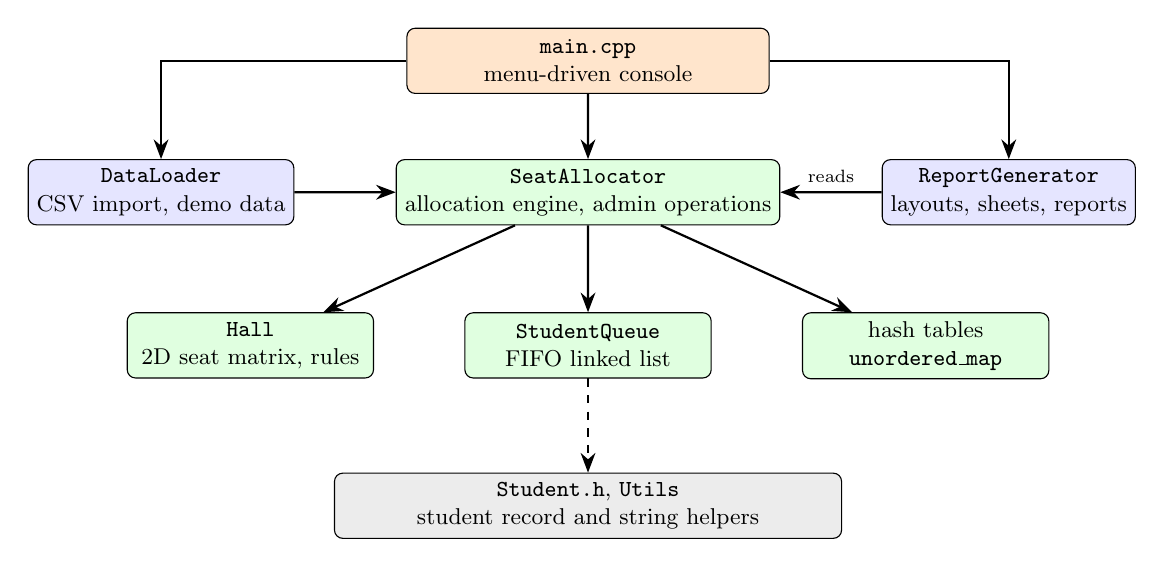
\begin{tikzpicture}[node distance=0.9cm and 0.7cm, scale=0.92, transform shape]
  \node (main)  [module, fill=orange!20, minimum width=5cm] {\texttt{main.cpp}\\ menu-driven console};
  \node (alloc) [module, below=of main, minimum width=5cm] {\texttt{SeatAllocator}\\ allocation engine, admin operations};
  \node (hall)  [module, below left=1.2cm and 0.3cm of alloc] {\texttt{Hall}\\ 2D seat matrix, rules};
  \node (queue) [module, below=1.2cm of alloc] {\texttt{StudentQueue}\\ FIFO linked list};
  \node (map)   [module, below right=1.2cm and 0.3cm of alloc] {hash tables\\ \texttt{unordered\_map}};
  \node (load)  [module, left=1.4cm of alloc, fill=blue!10] {\texttt{DataLoader}\\ CSV import, demo data};
  \node (rep)   [module, right=1.4cm of alloc, fill=blue!10] {\texttt{ReportGenerator}\\ layouts, sheets, reports};
  \node (base)  [module, below=1.3cm of queue, fill=gray!15, minimum width=7cm] {\texttt{Student.h}, \texttt{Utils}\\ student record and string helpers};
  \draw[arrow] (main) -- (alloc);
  \draw[arrow] (main.west) -| (load.north);
  \draw[arrow] (main.east) -| (rep.north);
  \draw[arrow] (load) -- (alloc);
  \draw[arrow] (rep) -- node[above, font=\scriptsize]{reads} (alloc);
  \draw[arrow] (alloc) -- (hall);
  \draw[arrow] (alloc) -- (queue);
  \draw[arrow] (alloc) -- (map);
  \draw[arrow, dashed] (queue) -- (base);
\end{tikzpicture}
\caption{Module diagram of SeatSync}
\end{figure}

\section{Flow Chart of the Seat Allocation}
The flow chart below shows what happens when the administrator chooses \emph{Run Seat Allocation}. It was drawn with TikZ so that it is part of the \LaTeX\ source and can be edited directly in Overleaf.

\begin{figure}[H]
\centering
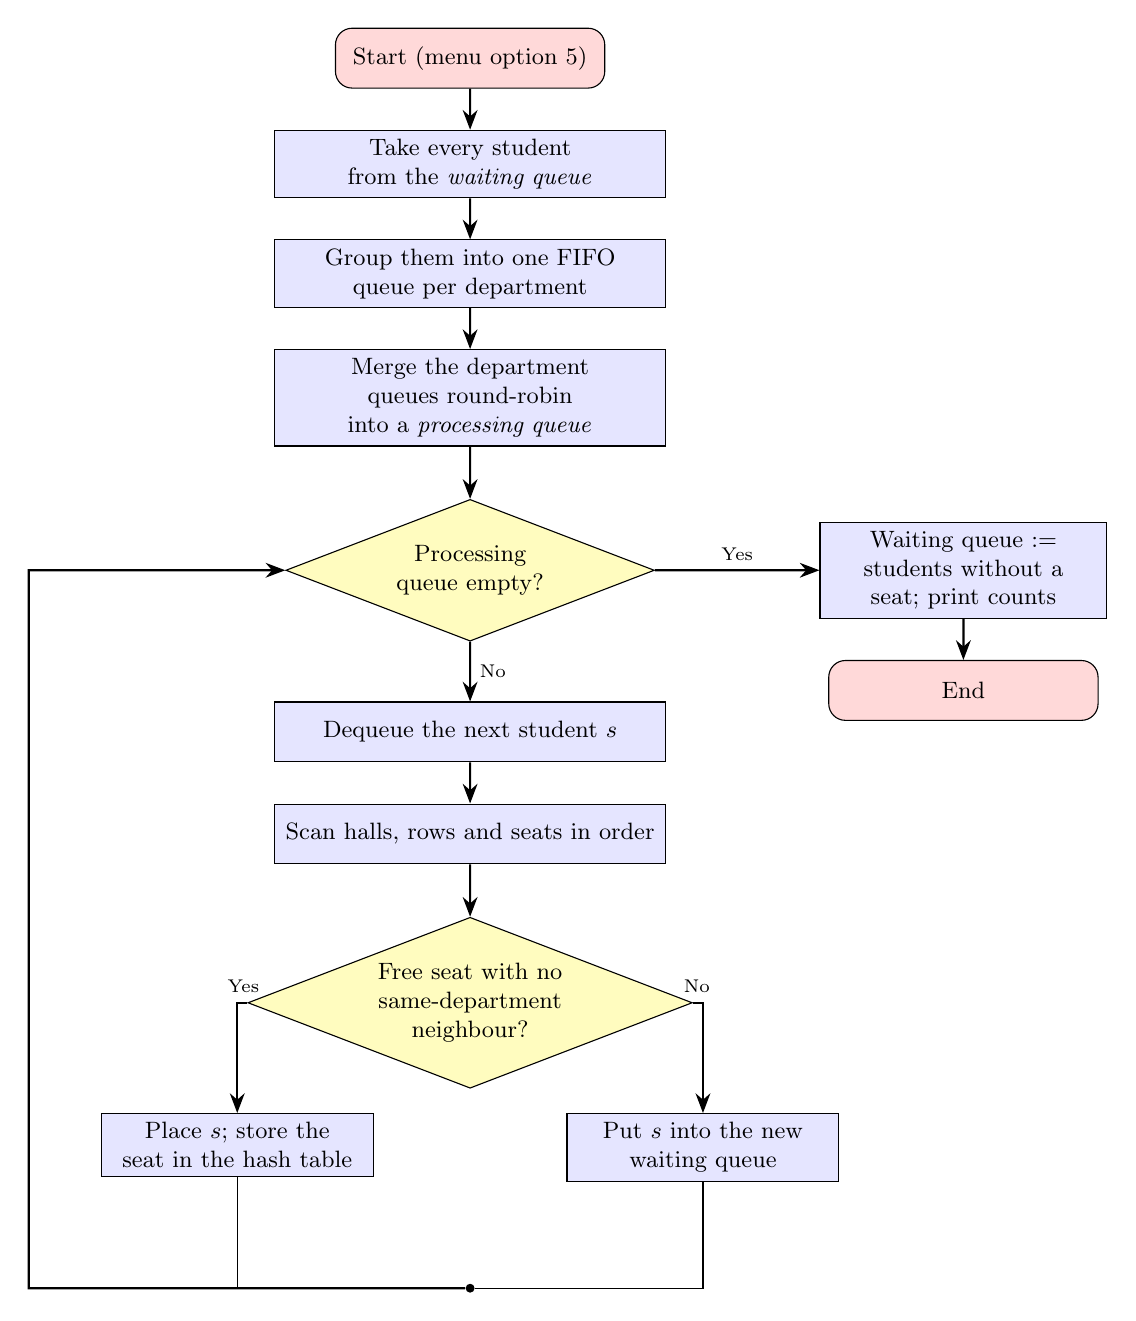
\begin{tikzpicture}[node distance=0.55cm, scale=0.95, transform shape]
  \node (start) [startstop] {Start (menu option 5)};
  \node (p1) [process, below=of start] {Take every student from the \emph{waiting queue}};
  \node (p2) [process, below=of p1] {Group them into one FIFO queue per department};
  \node (p3) [process, below=of p2] {Merge the department queues round-robin into a \emph{processing queue}};
  \node (d1) [decision, below=0.7cm of p3] {Processing queue empty?};
  \node (p4) [process, below=0.8cm of d1] {Dequeue the next student $s$};
  \node (p5) [process, below=of p4] {Scan halls, rows and seats in order};
  \node (d2) [decision, below=0.7cm of p5] {Free seat with no same-department neighbour?};
  \node (p6) [process, text width=3.4cm, below left=0.9cm and -0.2cm of d2] {Place $s$; store the seat in the hash table};
  \node (p7) [process, text width=3.4cm, below right=0.9cm and -0.2cm of d2] {Put $s$ into the new waiting queue};
  \node (m) [circle, fill=black, inner sep=1.2pt, below=0.9cm of d2, yshift=-1.7cm] {};
  \node (end1) [process, right=2.2cm of d1, text width=3.6cm] {Waiting queue := students without a seat; print counts};
  \node (end2) [startstop, below=of end1] {End};

  \draw[arrow] (start) -- (p1);
  \draw[arrow] (p1) -- (p2);
  \draw[arrow] (p2) -- (p3);
  \draw[arrow] (p3) -- (d1);
  \draw[arrow] (d1) -- node[right, font=\scriptsize]{No} (p4);
  \draw[arrow] (d1) -- node[above, font=\scriptsize]{Yes} (end1);
  \draw[arrow] (end1) -- (end2);
  \draw[arrow] (p4) -- (p5);
  \draw[arrow] (p5) -- (d2);
  \draw[arrow] (d2.west) -| node[above, pos=0.2, font=\scriptsize]{Yes} (p6.north);
  \draw[arrow] (d2.east) -| node[above, pos=0.2, font=\scriptsize]{No} (p7.north);
  \draw (p6.south) |- (m);
  \draw (p7.south) |- (m);
  \draw[arrow] (m) -- ++(-5.9cm,0) |- (d1.west);
\end{tikzpicture}
\caption{Flow chart of the allocation algorithm}
\end{figure}

\section{Working of the Modules}

\subsection{Student and Utils}
\texttt{Student} is a plain record with the registration number, name and department. \texttt{Utils} contains small helpers (trimming, upper-casing, splitting a CSV line, formatting text columns) that are shared by the other modules.

\subsection{StudentQueue -- the waiting line}
A singly linked list with a head and a tail pointer. \texttt{enqueue} adds a student at the tail and \texttt{dequeue} removes one from the head, both in $O(1)$. It is implemented from scratch (including copy and move constructors, so no memory is leaked or shared by accident). Three queues play a role:
\begin{itemize}
  \item the \textbf{waiting queue} holds every student who has no seat -- new registrations join at the back, which keeps registration order;
  \item one \textbf{department queue} per department, built temporarily at the start of an allocation;
  \item the \textbf{processing queue}, produced by serving the department queues in turn.
\end{itemize}
\emph{Why round-robin?} Suppose the waiting queue is CSE$_1$, CSE$_2$, CSE$_3$, ECE$_1$. Seating them in that order would put three CSE students next to each other. Serving the department queues alternately gives CSE$_1$, ECE$_1$, CSE$_2$, CSE$_3$, which interleaves the departments, while the students of each department still keep their registration order.

\subsection{Hall -- the seat matrix}
A hall is a \texttt{vector<vector<Seat>>} with \texttt{rows} $\times$ \texttt{cols} cells. A seat is \emph{free}, \emph{occupied} (storing the registration number and department) or \emph{blocked}. The central function is \texttt{placementProblem(r, c, dept, rules)}: it checks the four (or eight) neighbouring cells and returns either an empty string (the seat is legal) or a sentence explaining why not, e.g. ``Neighbouring seat A3 already has a EEE student (106125004)''. Because the matrix gives direct access to the neighbours, every check takes constant time. Seats are labelled by row letter and column number (\texttt{A1}, \texttt{B4}, \dots).

\subsection{SeatAllocator -- the engine}
It owns the list of halls, the student registry, the waiting queue and two hash tables: \texttt{regIndex} (registration number $\rightarrow$ student) and \texttt{seatOf} (registration number $\rightarrow$ hall, row, column).
\begin{itemize}
  \item \texttt{registerStudent} validates and normalises the data, rejects duplicates in $O(1)$ and enqueues the student.
  \item \texttt{allocatePending} runs the algorithm of the flow chart. Seats are searched \emph{first fit}: hall by hall, row by row, left to right; free seats left behind by the spacing rule are filled later by compatible students.
  \item \texttt{swapSeats}, \texttt{moveStudent}, \texttt{blockSeat}, \texttt{removeStudent} modify the plan. Each of them first tries the change; if a rule would be broken it restores the previous state (``undo'') and returns the reason, so the plan is \emph{never} left invalid.
  \item \texttt{blockSeat} on an occupied seat displaces the student and tries to re-seat him or her at once; if that is impossible the student returns to the waiting queue.
  \item \texttt{totalConflicts} counts adjacent same-department pairs and is used as a self-check after every allocation.
\end{itemize}

\subsection{DataLoader}
Reads a CSV file line by line, skipping comments, blank lines and the optional header. Every line is passed through \texttt{registerStudent}; duplicates and malformed lines are counted and reported with their line number. \texttt{generateDemoStudents} produces deterministic sample students for experiments.

\subsection{ReportGenerator}
All output functions take an \texttt{std::ostream}, so the same code prints to the screen and writes files. It draws the seat matrix, answers ``find my seat'', prints the waiting list, writes one attendance sheet per hall (sorted by registration number), prints the examination report (utilisation per hall, department-wise distribution, rule check) and exports the plan as CSV and TXT into the \texttt{output/} folder.

\subsection{main.cpp}
A menu loop with safe input handling: every input is read as a line and validated, wrong entries are re-asked, and the end of the input stream ends the program cleanly.

\section{Complexity}
Let $S$ be the number of students, $H$ the number of halls and $R\times C$ the size of a hall.
\begin{center}
{\small
\begin{tabular}{p{5.4cm}p{3.9cm}p{4.3cm}}
\toprule
\textbf{Operation} & \textbf{Structure} & \textbf{Time}\\
\midrule
enqueue / dequeue & \texttt{StudentQueue} & $O(1)$\\
check / place / vacate one seat & \texttt{Hall} (at most 8 neighbours) & $O(1)$\\
register student (duplicate check) & hash table & $O(1)$ average\\
find a student's seat & hash table & $O(1)$ average\\
group and merge department queues & queues & $O(S)$\\
find a seat for one student & first-fit scan & $O(H\cdot R\cdot C)$\\
complete allocation & all of the above & $O(S\cdot H\cdot R\cdot C)$ worst case\\
attendance sheet, $k$ students in a hall & sorting & $O(k\log k)$\\
\bottomrule
\end{tabular}}
\end{center}
For realistic sizes (a few thousand students and a few dozen halls) the allocation finishes instantly.

% =====================================================================
\chapter{Coding}
% =====================================================================

\section{Directory Structure}
The structure follows the project assignment.
\begin{verbatim}
DataSphere_106125127_106125129_106125131_106125133_CSLR31_Project/
|-- Makefile            build file
|-- a.out               compiled program
|-- README.md           user manual (read-me)
|-- include/            *.h  declarations
|     Student.h  Utils.h  StudentQueue.h  Hall.h
|     SeatAllocator.h  DataLoader.h  ReportGenerator.h
|-- Source/             *.cpp  definitions and main.cpp
|-- object/             *.o  object files
|-- data/               sample CSV files used by the test cases
|-- tests/              unit tests, scripted inputs/outputs
|-- Document/           report, user manual, test cases
|-- Video/              project experience video (.mp4)
\end{verbatim}

\section{Build}
\texttt{make} builds \texttt{a.out}; \texttt{make test} runs all tests; \texttt{make clean} removes the build products. The code is standard C++17 and compiles without warnings with \texttt{-Wall -Wextra}.

\section{Source Code}
The listings below are included directly from the source files, so the report always shows the code that was actually compiled and tested.

\subsection{Student and Utils}
\lstinputlisting[style=cpp, caption={include/Student.h}]{../include/Student.h}
\lstinputlisting[style=cpp, caption={include/Utils.h}]{../include/Utils.h}
\lstinputlisting[style=cpp, caption={Source/Utils.cpp}]{../Source/Utils.cpp}

\subsection{StudentQueue}
\lstinputlisting[style=cpp, caption={include/StudentQueue.h}]{../include/StudentQueue.h}
\lstinputlisting[style=cpp, caption={Source/StudentQueue.cpp}]{../Source/StudentQueue.cpp}

\subsection{Hall}
\lstinputlisting[style=cpp, caption={include/Hall.h}]{../include/Hall.h}
\lstinputlisting[style=cpp, caption={Source/Hall.cpp}]{../Source/Hall.cpp}

\subsection{SeatAllocator}
\lstinputlisting[style=cpp, caption={include/SeatAllocator.h}]{../include/SeatAllocator.h}
\lstinputlisting[style=cpp, caption={Source/SeatAllocator.cpp}]{../Source/SeatAllocator.cpp}

\subsection{DataLoader}
\lstinputlisting[style=cpp, caption={include/DataLoader.h}]{../include/DataLoader.h}
\lstinputlisting[style=cpp, caption={Source/DataLoader.cpp}]{../Source/DataLoader.cpp}

\subsection{ReportGenerator}
\lstinputlisting[style=cpp, caption={include/ReportGenerator.h}]{../include/ReportGenerator.h}
\lstinputlisting[style=cpp, caption={Source/ReportGenerator.cpp}]{../Source/ReportGenerator.cpp}

\subsection{Main Program}
\lstinputlisting[style=cpp, caption={Source/main.cpp}]{../Source/main.cpp}

\subsection{Build File}
\lstinputlisting[style=cpp, language={}, caption={Makefile}]{../Makefile}

% =====================================================================
\chapter{Testing}
% =====================================================================

\section{Testing Strategy}
Testing was done on three levels.
\begin{enumerate}
  \item \textbf{Unit tests} (\texttt{tests/test\_core.cpp}, 91 checks): the queue (FIFO order, empty queue, copying), the hall (neighbour rules with and without diagonals, blocked and occupied seats, seat labels), the allocator (registration validation, allocation, overflow, clearing, swap, move, block, remove) and the CSV loader.
  \item \textbf{Scripted test cases} (7): complete sessions typed into the real program. The input of each is stored in \texttt{tests/inputs/}, the expected console output in \texttt{tests/expected/}; \texttt{sh tests/run\_tests.sh} replays all of them and compares.
  \item \textbf{Self-check inside the program}: after every allocation the number of rule conflicts is recomputed independently (\texttt{totalConflicts}) and shown. It was 0 in every test.
\end{enumerate}
Because the allocation uses no random numbers, results are reproducible.

\section{Test Data}
\begin{center}
\begin{tabular}{ll}
\toprule
\textbf{File} & \textbf{Content}\\
\midrule
\texttt{students\_sample.csv} & 15 students, 5 departments\\
\texttt{students\_overflow.csv} & 25 students, more than two small halls can hold\\
\texttt{students\_dominant.csv} & 12 students: 9 CSE + 3 ECE (stress test for the rule)\\
\texttt{students\_errors.csv} & duplicate, missing field, bad number, empty name\\
\bottomrule
\end{tabular}
\end{center}

\section{Summary of Test Cases}
\begin{center}
\begin{tabular}{clp{7.6cm}c}
\toprule
\textbf{\#} & \textbf{Test case} & \textbf{What is checked} & \textbf{Result}\\
\midrule
1 & Basic allocation & 15 students in one 4$\times$5 hall, seat look-up, unknown student & Pass\\
2 & Overflow, several halls & 25 students, 21 seats: 4 wait; adding a hall seats them & Pass\\
3 & Dominant department & 9 CSE + 3 ECE; normal rule vs.\ diagonal rule & Pass\\
4 & Administrator changes & swap, move, block, unblock, remove; rejections with reasons & Pass\\
5 & CSV and registration errors & duplicates, malformed lines, invalid entries & Pass\\
6 & Input validation & wrong menu input, bad hall sizes, invalid seats, empty hall list & Pass\\
7 & Reports and export & attendance sheets, examination report, CSV/TXT files & Pass\\
\bottomrule
\end{tabular}
\end{center}
Unit tests: 91 passed, 0 failed. Scripted tests: 7 passed, 0 failed.

\section{Observations}
\begin{itemize}
  \item \textbf{Test 1:} the round-robin order spreads the five departments over the hall; no two equal departments touch.
  \item \textbf{Test 2:} the first run seats 21 students and keeps 4 CSE/ECE students in the queue; after \texttt{Hall-C} is added the next run processes \emph{only} the waiting students.
  \item \textbf{Test 3:} when one department makes up three quarters of the students, the spacing rule cannot be satisfied for everybody (a $3\times4$ hall can hold at most 6 CSE students under the basic rule). SeatSync does not break the rule; the remaining students stay in the queue. The diagonal rule is stricter and seats 7 instead of 9 students.
  \item \textbf{Test 4:} a swap that would put an EEE student beside another EEE student is rejected and both students stay where they were. Blocking an occupied seat re-seats the student immediately.
  \item \textbf{Tests 5 and 6:} no input can crash the program; every error produces a clear message.
\end{itemize}

\section{Console Transcripts}
The repeated main menu is removed from the transcripts to save space. Lines after a prompt show what the tester typed.

\subsection*{Test case 1 -- basic allocation}
\lstinputlisting[style=log]{testlogs/tc1_basic_allocation.txt}
\subsection*{Test case 2 -- overflow and several halls}
\lstinputlisting[style=log]{testlogs/tc2_overflow_multiple_halls.txt}
\subsection*{Test case 3 -- dominant department and diagonal rule}
\lstinputlisting[style=log]{testlogs/tc3_dominant_department.txt}
\subsection*{Test case 4 -- administrator modifications}
\lstinputlisting[style=log]{testlogs/tc4_admin_changes.txt}
\subsection*{Test case 5 -- CSV loading and registration}
\lstinputlisting[style=log]{testlogs/tc5_csv_and_registration.txt}
\subsection*{Test case 6 -- input validation}
\lstinputlisting[style=log]{testlogs/tc6_input_validation.txt}
\subsection*{Test case 7 -- reports and export}
\lstinputlisting[style=log]{testlogs/tc7_reports_and_export.txt}

% =====================================================================
\chapter{Contributions, Key Takeaways and Future Scope}
% =====================================================================

\section{Individual Contributions}
\todo{The assignment asks for a candid account. The split below is only a proposal that matches the module structure -- replace it with what each member really did.}

\begin{itemize}
  \item \textbf{S Vijayakrishna (106125127)} -- \todo{e.g.\ \texttt{StudentQueue}: linked-list queue, round-robin merge of department queues}
  \item \textbf{Tanishaa E A (106125129)} -- \todo{e.g.\ \texttt{Hall}: seat matrix, spacing rules, seat labels}
  \item \textbf{Torim Chakma (106125131)} -- \todo{e.g.\ \texttt{SeatAllocator}: allocation algorithm, swap/move/block operations}
  \item \textbf{Vadlakonda Sathwika (106125133)} -- \todo{e.g.\ \texttt{DataLoader}, \texttt{ReportGenerator}, \texttt{main.cpp}, testing and documentation}
\end{itemize}

\section{Key Takeaways}
\begin{itemize}
  \item A \textbf{queue} is the natural tool for ``first come, first served'' processing; building it ourselves (with correct copy and move behaviour) gave a deep understanding of pointers and memory ownership.
  \item A \textbf{2D matrix} turns a spatial rule (``not next to each other'') into a constant-time neighbour check.
  \item A \textbf{hash table} makes look-ups and duplicate detection instant, compared with scanning a list.
  \item \textbf{Try, then undo:} every modification is validated first and rolled back on failure, so the plan can never become invalid; a separate conflict counter verifies this independently.
  \item \textbf{Separate declarations from definitions} (\texttt{.h} / \texttt{.cpp}), write unit tests and scripted tests early, and the rest of the project (debugging, documentation, demo) becomes much easier.
\end{itemize}

\section{Future Scope}
\begin{itemize}
  \item Integration with the campus ERP so that registration data are imported automatically instead of through CSV files.
  \item A real-time \textbf{absence reassignment} module that re-optimises empty seats on the day of the exam.
  \item Seating rules per course and per exam session (e.g.\ avoiding students who write the same paper beside each other), and several exam sessions per day.
  \item A graphical or web front end for administrators and a mobile ``find my seat'' page for students.
  \item Smarter placement strategies (for example balancing the load over all halls or searching for the best seating with backtracking).
  \item Printing seat labels and invigilator duty lists automatically.
\end{itemize}

\chapter{Acknowledgement}
We would like to express our sincere gratitude to our faculty, \textbf{\facultyname}, for his guidance, encouragement and the freedom to choose a problem that matters to us. The Data Structures Laboratory gave us the opportunity to apply queues, matrices and hash tables to a real problem of our own campus. We also thank the Department of Computer Science and Engineering, NIT Tiruchirappalli, for the laboratory facilities, and our classmates who tested the program and gave honest feedback.

\chapter{References}
\begin{itemize}
  \item T.~H.~Cormen, C.~E.~Leiserson, R.~L.~Rivest, C.~Stein, \textit{Introduction to Algorithms}, MIT Press -- queues, hash tables, complexity analysis.
  \item M.~A.~Weiss, \textit{Data Structures and Algorithm Analysis in C++}, Pearson -- linked-list queues, hashing.
  \item B.~Stroustrup, \textit{The C++ Programming Language}, Addison-Wesley -- copy and move semantics, STL.
  \item C++ reference documentation for \texttt{std::unordered\_map}, \texttt{std::filesystem} and \texttt{std::vector}: \url{https://en.cppreference.com}
  \item GNU Make manual: \url{https://www.gnu.org/software/make/manual/}
  \item UNESCO and the United Nations, Sustainable Development Goals: \url{https://www.unesco.org/en/sdgs}, \url{https://sdgs.un.org/goals/goal4}, \url{https://sdgs.un.org/goals/goal9}
  \item Overleaf documentation on \LaTeX, TikZ and the \texttt{listings} package: \url{https://www.overleaf.com/learn}
\end{itemize}

\end{document}
